% This is samplepaper.tex, a sample chapter demonstrating the
% LLNCS macro package for Springer Computer Science proceedings;
% Version 2.20 of 2017/10/04
%
\documentclass[runningheads,custombib]{llncs}
%
\usepackage{graphicx}
% Used for displaying a sample figure. If possible, figure files should
% be included in EPS format.
%
% If you use the hyperref package, please uncomment the following line
% to display URLs in blue roman font according to Springer's eBook style:
% \renewcommand\UrlFont{\color{blue}\rmfamily}

%my package
\usepackage[backend=biber,
%this is the label style in the bibliography at the end of document
style=numeric,
%this is the label style for each citation in the document
citestyle=numeric,
sorting=none,
%sortcae=false                  
%citestyle=authoryear
]{biblatex}
%\usepackage[backend=biber]{biblatex}
\addbibresource{paper.bib} %Imports bibliography file

\usepackage{amsmath}
\usepackage{amsfonts}

\usepackage{tikz}
\usetikzlibrary{chains,shapes.multipart}
\usepackage{pgf}
\usepackage{tikz}
\usetikzlibrary{arrows,automata}




\begin{document}
%
\title{Continuous-Time Markov Chain with Alarms analysis and comparaison of tools \thanks{Supported by organization x.}}
%
%\titlerunning{Abbreviated paper title}
% If the paper title is too long for the running head, you can set
% an abbreviated paper title here
%
\author{Thomas Mari\inst{1}\orcidID{0000-1111-2222-3333} \and
Second Author\inst{2,3}\orcidID{1111-2222-3333-4444} \and
Third Author\inst{3}\orcidID{2222--3333-4444-5555}}
%
\authorrunning{F. Author et al.}
% First names are abbreviated in the running head.
% If there are more than two authors, 'et al.' is used.
%
\institute{Princeton University, Princeton NJ 08544, USA \and
Springer Heidelberg, Tiergartenstr. 17, 69121 Heidelberg, Germany
\email{lncs@springer.com}\\
\url{http://www.springer.com/gp/computer-science/lncs} \and
ABC Institute, Rupert-Karls-University Heidelberg, Heidelberg, Germany\\
\email{\{abc,lncs\}@uni-heidelberg.de}}
%
\maketitle              % typeset the header of the contribution
%
\begin{abstract}
	Phase-type fitting remains the only way of modeling non-Markovian distributions within PRISM model checker.
	When analyzing models with phase-type distributions, it is problematic to obtain results of sufficient precision within reasonable time.
	We ran experimental computations and deduced a reliable way of obtaining precise analysis results for phase-type fitted PRISM CTMCs.
	Lastly, we hint at an entirely different (and arguably better) approach to handling non-Markovian distributions.

The abstract should briefly summarize the contents of the paper in
150--250 words.

\keywords{PRISM model checker \and CTMC \and deterministic timeout \and phase-type distribution \and modeling \and analysis  \and Second keyword \and Another keyword.}
\end{abstract}
%
%
%
\section{Introduction}

	PRISM \cite{KNP11} and Storm \cite{DBLP:journals/corr/DehnertJK017} are popular tools for modeling and analysis of stochastic systems in continuous time. They use efficient algorithms for analysis of continuous time Markov chains (CTMC). This approach suffers from a severe restriction of modeling power --- the time between transitions must be exponentially distributed. This restriction can be remedied by the use of phase-type distributions, which can approximate any general distribution with arbitrary accuracy by only using exponential distributions \cite{Buchholz:2014:IMP:2683922}. However, the use of phase-type distributions drastically increases the number of states within the CTMC.
	
	In this paper, we experimentally evaluate the precision of the result and required computation time of various approaches to analysis of continuous time stochastic models with deterministic transitions (timeouts). The obtained results are then compared against results of our extension of PRISM capable of efficiently analyzing CTMC with non-Markovian alarms (ACTMC).
	
	
\subsection{Time distribution}
The model we use are probabilistic continuous time model, which means that the time passed in a state will depend on a time distribution. A time distribution can be depicted by its cumulative distribution function (CDF) $F : \mathbb{R} \rightarrow[0,1]$, $F(t)$ is the probability that the event will happend before the time $t$. The exponential distribution of rate $\lambda$ has a CDF $F(t) = 1 - \exp(-\lambda t)$, it is important to keep in mind that a rate refers to the exponential distribution. The Dirac distribution of timeout $\tau$ has a CDF $F(t) = \chi_{[\tau,+\infty[}(t) = 
\left\{
	\begin{array}{l}
		0 \text{ if } t < \tau\\
		1\text{ else}
	\end{array}
\right.$. In this paper, time distribution which are not exponential will be called non-Markovian distribution.
\subsection{CTMC}
A continuous-time Markov chain (CTMC) is a triple $C = (S,Q,s_{in})$, where 
\begin{itemize}
	\item[$\bullet$] S is a finite set of states
	\item[$\bullet$] $Q : S \times S \rightarrow \mathbb{R}_{\geq 0}$ is a matrix of rates such that $\sum_{s' \in S} Q(s,s')  > 0$ for each $s \in S$
	\item[$\bullet$] $s_{in} \in S$ is an initial state
\end{itemize} 
$Q(s,s')$ is the rate of the transition from $s$ to $s'$.
We define the exit rate of state $s$ as $\lambda_s = \sum_{s' \in S} Q(s,s')$

A run of a CTMC $\mathcal{C}$ is an infinite alternating sequence of states and times $\omega = s_0t_0s_1t_1...$ where 
\begin{itemize}
	\item[$\bullet$] $s_0 = s_{in}$
	\item[$\bullet$] $s_i$ is the i-th state
	\item[$\bullet$] $t_i$ is the time spent in $s_i$
\end{itemize}

For each $i \in \mathbb{N}$ \begin{itemize}
	\item[$\bullet$] $t_i$ is choosen randomly according to the exponential distribution with rate $\lambda_{s_i}$
	\item[$\bullet$] $s_{i+1}$ is choosen according to the discrete distribution $\dfrac{Q(s_i,.)}{\lambda_{s_i}}$
\end{itemize}

\subsection{ACTMC}

Continuous-Time Markov Chain with Alarms (ACTMC)s. I won't give the formal semantics which might not fit in this paper. We can see ACTMC as CTMC with some events called alarms that are enabled in disjoints sets of states and those events has their own timer which is active only when inside the enabled set and happend according to some continuous time distribution. Those alarms works concurrently with the exponential transition seen in the CTMC.

$\mathcal{A} = (S,Q,s_{in},A,\langle S_a \rangle,\langle P_a \rangle,\langle F_a \rangle)$
where :
\begin{itemize}
	\item[$\bullet$]$(S,Q,s_{in})$ is a CTMC
	\item[$\bullet$] $A$ is a set of alarms
	\item[$\bullet$] $\langle S_a \rangle = (S_a)_{a \in A}$, the set of states where $a$ is enabled
		\begin{itemize}
			\item[$\bullet$] if $a \neq a'$ then $S_a \bigcap S_{a'} = \emptyset$ 
		\end{itemize}
	\item[$\bullet$]$\langle P_a \rangle = (P_a)_{a \in A}$ where $P_a$ is a probability matrix
	\item[$\bullet$]$\langle F_a \rangle = (F_a)_{a \in A}$ where $F_a$ is a cumulative distribution function (CDF) 
\end{itemize}

Operational Behavior

A run of a ACTMC $\mathcal{A}$ is an infinite alternating sequence of states and times $(s_0,\eta_0)t_0(s_1,\eta_1)t_1...$ where 
\begin{itemize}
	\item[$\bullet$] $s_0 = s_{in}$
	\item[$\bullet$] $s_i$ is the i-th state
	\item[$\bullet$] $t_i$ is the delay in $s_i$, $t_i$ is the time spent in $s_i$ without alarms
	\item[$\bullet$] $\eta_i$ is the value of the timer, the remaining time for the alarm to ring.
\end{itemize}
We define $S_{off} = S\setminus\bigcup_{a \in A} S_a$ the set of states where no alarms are enabled

For initialization
\begin{itemize}
	\item[$\bullet$] $s_0 = s{in}$
	\item[$\bullet$] $\eta_0 =$
	$\left\{
		\begin{array}{l}
		\infty \text{ if } s_0 \in S_{off}\\
		 \text{randomly choosen according to }F_a\text{ if } s_0 \in S_{a}
		\end{array}
		\right.$ 
\end{itemize}
For each $i \in \mathbb{N}, t_i$ is choosen randomly according to the exponential distribution $\lambda_{s_i}$

Two cases are possible, either the alarm ring ($\eta_i \leq t_i$) or $t_i$ is too short and the alarm doesn't ring.

If $\eta_i \leq t_i$, the alarm ring
\begin{itemize}
	\item[$\bullet$] $t_i := \eta_i$ the value of delay is overwritten and match the time spent in $s_i$
	\item[$\bullet$] $s_{i+1}$ is choosen according to the discrete distribution $P_a(s_i,.)$
	\item[$\bullet$] $\eta_{i+1} =$
	$\left\{
	\begin{array}{l}
		\infty \text{ if } s_{i+1} \in S_{off}\\
		\text{randomly choosen according to }F_a\text{ if } s_{i+1} \in S_{a}
	\end{array}
	\right.$ 
\end{itemize}

If $\eta_i > t_i$, the alarm does not ring
\begin{itemize}
	\item[$\bullet$] $t_i$ the value of delay remain the same and match the time spent in $s_i$
\item[$\bullet$] $s_{i+1}$ is choosen according to the discrete distribution $\dfrac{Q(s_i,.)}{\lambda_{s_i}}$
	\item[$\bullet$] $\eta_{i+1} =$
	$\left\{
	\begin{array}{l}
	\infty \text{ if } s_{i+1} \in S_{off}\\
	\eta_i - t\text{ if }s_{i+1} \in S_{a}\text{ and }s_{i} \in S_{a}\\
	\text{randomly choosen according to }F_a\text{ if }s_{i+1} \in S_{a}\text{ and }s_{i} \notin S_{a}
	\end{array}
	\right.$ 
\end{itemize}
 If the state remain in the set enabled by the alarm, it is updated. Otherwise it is reset according to the new enabled set.
 
\subsection{Phase Type fitting}
Phase Type fitting (PH fitting) is approaching a non-Markovian distribution by a sequence of exponential distributions. 
Consider an infinite sequence of finite sequences of rates of length k $((\lambda_{i,k})_{i=0}^{k})_{k \in \mathbb{N}}$. We want that the distribution of the sequence of exponential transitions to converge to the non-Markovian distribution.

To obtain analysis on ACTMC, we use PH fitting to create CTMC from ACTMC, and analyse those CTMC Then we deduce results on the ACTMC.  The reason is that Prism or Storm can use CTMC and not ACTMC. Figure \ref{fig:simple_actmc} and figure \ref{fig:simple_ctmc} are a toy example of the PH fitting of a simple ACTMC $\mathcal{A} = (\{A,B\},
\begin{bmatrix}
	0.5       & 0 \\
	2       & 1 
\end{bmatrix}
,A,\{A\},
\begin{bmatrix}
1       & 0
\end{bmatrix}
,\{d\})$ with constant parameter $k$. The created CTMC is $\mathcal{C} = (\{A,B,1,2,...,k-1,B\},
\begin{bmatrix}
0       & \lambda_{1,k} 	& 0		& 0		& ...		& 0\\
0       & 0 	& \lambda_{2,k}		& 0		& ...		& 0\\
0       & 0 	& 0		& \lambda_{3,k}		& ...		& 0\\
0       & 0 	& 0		& 0		& ...		& 0\\
...       & ... 	& ...		& ...		& ...		& \lambda_{k,k}\\
0       & 0 	& 0		& 0		& 0		& 0
\end{bmatrix}
,A)$






EXIT RATE > 0 §!!!!!!!!!!!!!!!!!!!!!!!!!!!!!!
	\begin{figure}
		\centering
		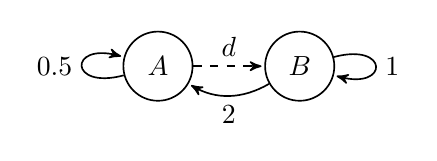
\begin{tikzpicture}[->,>=stealth',shorten >=1pt,auto,node distance=1.80cm,
		semithick]
		\tikzstyle{every state}=[fill=white,draw=black,text=black]
		
		\node[state] (s0)                    {$A$};
		\node[state]         (sn) [right of=s0]       {$B$};
		\path[->, dashed]
		(s0) edge 	node {$d$} (sn);
		\path[->]
		(s0) edge [loop left]	node {0.5} (s0)
			
		(sn) edge [bend left]	node {2} (s0)
		edge [loop right]	node {1} (sn);			
		\end{tikzpicture}
		\caption{Model of a simple ACTMC $\mathcal{A}$, $d$ is a non-Markovian distribution.}
		\label{fig:simple_actmc}
	\end{figure}
	
	\begin{figure}
		\centering
		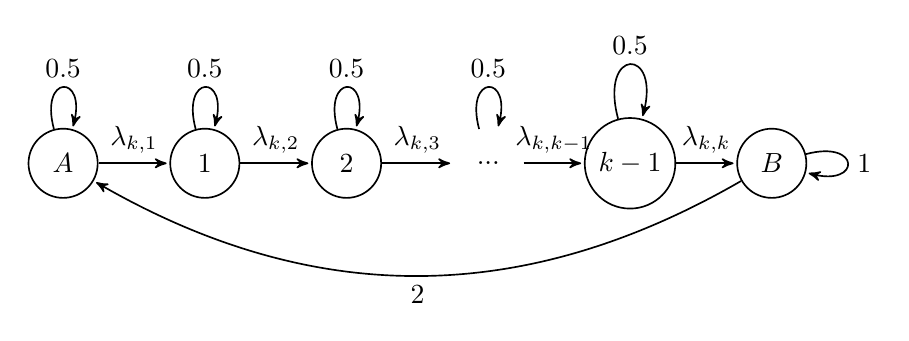
\begin{tikzpicture}[->,>=stealth',shorten >=1pt,auto,node distance=1.80cm,
		semithick]
		\tikzstyle{every state}=[fill=white,draw=black,text=black]
		
		\node[state] (s0)                    {$A$};
		\node[state]         (s1) [right of=s0] {$1$};
		\node[state]         (s2) [right of=s1] {$2$};
		\node[state,draw=none]         (s4) [right of=s2]       {$...$};
		\node[state]         (sw) [right of=s4,fill=white,text=black]       {$k-1$};
		\node[state]         (sn) [right of=sw]       {$B$};
		
		
		
		\path[->]  
		(s0) edge	node {$\lambda_{k,1}$} (s1)
			edge [loop above]	node {0.5} (s0);
		\path[->]
	
		[->]
		(s1) edge	node {$\lambda_{k,2}$} (s2)
			edge [loop above]	node {0.5} (s1);
		\path[->]
	
	
		(s2) edge   node {$\lambda_{k,3}$} (s4)
			edge [loop above]	node {0.5} (s2);
		\path[->]
	
	
		(s4) edge   node {$\lambda_{k,k-1}$} (sw)
			edge [loop above]	node {0.5} (s4);
		\path[->]
	
	
		(sw) edge   node {$\lambda_{k,k}$} (sn)
			edge [loop above]	node {0.5} (sw);
		\path[->]
		
		(sn) edge [bend left]	node {2} (s0)
		edge [loop right]	node {1} (sn);
		\end{tikzpicture}
		\caption{Model of a CTMC obtain by PH fitting of the ACTMC figure \ref{fig:simple_actmc}.}
		\label{fig:simple_ctmc}
	\end{figure}

\section{Related Work}
Maybe talk about the previous work of vojta and lubosh

\section{Contribution}
\subsection{A Subsection Sample}
Please note that the first paragraph of a section or subsection is
not indented. The first paragraph that follows a table, figure,
equation etc. does not need an indent, either.

Subsequent paragraphs, however, are indented.

\subsubsection{Sample Heading (Third Level)} Only two levels of
headings should be numbered. Lower level headings remain unnumbered;
they are formatted as run-in headings.

\paragraph{Sample Heading (Fourth Level)}
The contribution should contain no more than four levels of
headings. Table~\ref{tab1} gives a summary of all heading levels.

\begin{table}
\caption{Table captions should be placed above the
tables.}\label{tab1}
\begin{tabular}{|l|l|l|}
\hline
Heading level &  Example & Font size and style\\
\hline
Title (centered) &  {\Large\bfseries Lecture Notes} & 14 point, bold\\
1st-level heading &  {\large\bfseries 1 Introduction} & 12 point, bold\\
2nd-level heading & {\bfseries 2.1 Printing Area} & 10 point, bold\\
3rd-level heading & {\bfseries Run-in Heading in Bold.} Text follows & 10 point, bold\\
4th-level heading & {\itshape Lowest Level Heading.} Text follows & 10 point, italic\\
\hline
\end{tabular}
\end{table}


\noindent Displayed equations are centered and set on a separate
line.
\begin{equation}
x + y = z
\end{equation}
Please try to avoid rasterized images for line-art diagrams and
schemas. Whenever possible, use vector graphics instead (see
Fig.~\ref{fig1}).

\begin{figure}
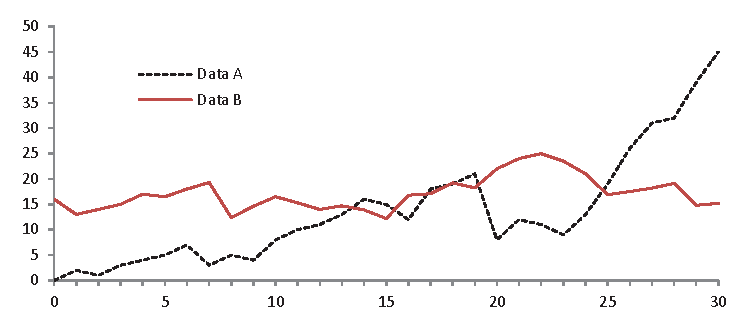
\includegraphics[width=\textwidth]{fig1.eps}
\caption{A figure caption is always placed below the illustration.
Please note that short captions are centered, while long ones are
justified by the macro package automatically.} \label{fig1}
\end{figure}

\begin{theorem}
This is a sample theorem. The run-in heading is set in bold, while
the following text appears in italics. Definitions, lemmas,
propositions, and corollaries are styled the same way.
\end{theorem}
%
% the environments 'definition', 'lemma', 'proposition', 'corollary',
% 'remark', and 'example' are defined in the LLNCS documentclass as well.
%
\begin{proof}
Proofs, examples, and remarks have the initial word in italics,
while the following text appears in normal font.
\end{proof}
For citations of references, we prefer the use of square brackets
and consecutive numbers. Citations using labels or the author/year
convention are also acceptable. The following bibliography provides
a sample reference list with entries for journal
articles~\cite{ref_article1}, an LNCS chapter~\cite{ref_lncs1}, a
book~\cite{ref_book1}, proceedings without editors~\cite{ref_proc1},
and a homepage~\cite{ref_url1}. Multiple citations are grouped
\cite{ref_article1,ref_lncs1,ref_book1},
\cite{ref_article1,ref_book1,ref_proc1,ref_url1}.
\section{Conclusion}
%
% ---- Bibliography ----
%
% BibTeX users should specify bibliography style 'splncs04'.
% References will then be sorted and formatted in the correct style.
%
% \bibliographystyle{splncs04}
% \bibliography{mybibliography}

\begin{thebibliography}{8}
\bibitem{ref_article1}
Author, F.: Article title. Journal \textbf{2}(5), 99--110 (2016)

\bibitem{ref_lncs1}
Author, F., Author, S.: Title of a proceedings paper. In: Editor,
F., Editor, S. (eds.) CONFERENCE 2016, LNCS, vol. 9999, pp. 1--13.
Springer, Heidelberg (2016). \doi{10.10007/1234567890}

\bibitem{ref_book1}
Author, F., Author, S., Author, T.: Book title. 2nd edn. Publisher,
Location (1999)

\bibitem{ref_proc1}
Author, A.-B.: Contribution title. In: 9th International Proceedings
on Proceedings, pp. 1--2. Publisher, Location (2010)

\bibitem{ref_url1}
LNCS Homepage, \url{http://www.springer.com/lncs}. Last accessed 4
Oct 2017

\printbibliography

\end{thebibliography}
\end{document}
